\chapter{Methods}

\section{Domain Description}
As stated before the application should provide a time-tracking solution for commercial projects.
Therefore it is divided into three general areas:
\begin{itemize}
\item \textbf{Project}: A project is the overall term for a distinguishable amount of work that is done for a specific customer.
\item \textbf{Phase}: Each project exists of one or more phases that are used to monitor the progress of the project.
\item \textbf{Activity}: A activity represents a workload that is done by a specific member in a specific phase for a specific project.
\end{itemize}
In order to be able to safely administer the system, three roles of members exist:
\begin{itemize}
\item \textbf{Administrator}: This member is responsible for creating and deleting users, resetting passwords and is allowed to perform all actions to project, phases, ect.
\item \textbf{Project Leader}: A project leader has the responsibility of maintaining project specific data, such as description, phases and assigning project members. He is \emph{not} allowed to create new users. After creating a new project, one is automatically project leader. A project leader is allowed to monitor the statistics of his projects including the workloads of the project members
\item \textbf{Member}: As a simple member one is allowed to add, delete and modify activities created by the user. A member is only allowed to perform this actions for projects he is assigned to. He is also only allowed to monitor his own statistics.
\end{itemize}

\subsection{Use-Cases}
\subsubsection{General Use-Cases}
\begin{enumerate}
\item \textbf{Login:} After starting the program, a login prompt shall show up. The user provides his credentials which will be compared to the saved credentials in the database. If they are correct, he is forwarded to the main program.\\
The user has the possibility to reset his password by activating a button and providing his email-address. A new password will be sent to the address, if a user with this address is known by the system. 

\item \textbf{Starting / Stopping activities:} Through a banner at the top of the program each user can select a project he is assigned to and furthermore a phase of this project. After providing a name of the activity he can start the activity by clicking on a start button. The same button can be used to stop the activity. After stopping (or closing the application), the activity is complete and is added to the database and project statistics.

\item \textbf{Personal statistics:} Utilizing the associated button of the left side bar the main panel lists all project the user is assigned to and the time he spent working for these projects. At the top of the main panel he can choose the period he wants to see. After clicking on one of the entries a statistic of the working time for each phase of the project is shown. By clicking at a phase all activities in this phase are listed and can be modified and deleted, furthermore a new activity can be created here too. By clicking on a button at the top the user can switch the view to the previous view.

\item \textbf{Create and manage projects:} Each user can create new projects by using the associated button of the left side bar. The main panel then lists all projects which project leader he is. After clicking on a entry, the main window shows the details of the project, such as the description, the created phases and the project members. He is able to perform all necessary operations associated with the project in this view, as well as declaring a new project leader.

\item \textbf{Settings:} Utilizing the associated button of the left side bar the main panel provides means to change the password, email-address and name.
\end{enumerate}
\subsubsection{Project leader Use-Cases}
\begin{enumerate}
\item \textbf{Project statistics:} Other than normal users, a project leader can monitor the statistics of all of his projects by using the according button on the side bar. The main panel lists all projects he is leader of. After choosing one project he can choose the period he is interested in at the top of the panel. At the left side of the main window now all project members are listed. After choosing one or more project members, the time they spent working for the different phases of the project is listed at the center.
\end{enumerate}


\subsubsection{Administrator Use-Cases}
\begin{enumerate}
\item \textbf{Manage Projects:} As administrator it is possible to manage \emph{all} projects as he would be project leader.
\item \textbf{Manage Users:} By clicking on the associated button, users can be managed, e.g. changing their passwords or create new users.
\end{enumerate}


The persistent storage has a quite simple structure, as can be seen in figure \ref{fig:database}. It is notable that the roles are described as text and therefore are human-readable. 
\begin{figure}[htbp]
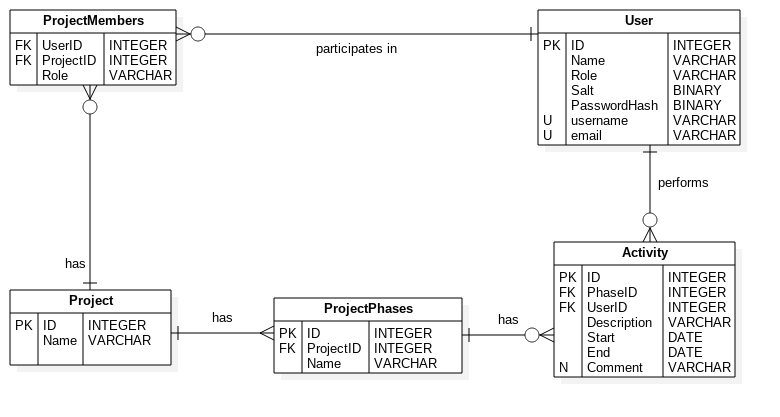
\includegraphics[width=\textwidth]{./content/pictures/database.png}
\caption{Database diagram}
\label{fig:database}
\end{figure}

\clearpage

\section{Phase 1: One Databse and UI}
\subsection{Monolithic Code Samples}
%\subsubsection{Database Access}
%\subsubsection{UI Interaction}

\subsection{Best-Practice Code Samples}
%\subsubsection{Database Access}
%\subsubsection{UI Interaction}

\section{Phase 2: More Databases / UIs}

\subsection{Monolithic Code Samples}
%\subsubsection{Database Access}
%\subsubsection{UI Interaction}

\subsection{Best-Practice Code Samples}
%\subsubsection{Database Access}
%\subsubsection{UI Interaction}